\chapter{Architecture}

This chapter describes the architecture of JPaxos.
First the general architecture of the library is presented, consecutively focusing on its parts in detail.
Later the most significant data structures and the threading architecture details are presented.

\section{Architecture overview}
\indent\par
The easiest way to understand the architecture of JPaxos is to analyze its architecture in top-down approach.

\subsection{Processes and their communication}

For JPaxos there are two possible approaches of building replicated services. The first, recommended by us, 
requires from the service client application using a \texttt{Client} module. % TODO not English
The other approach incorporates the client module within replica, but 
it places the responsibility for finding a working replica on the user. % TODO rewrite
The possible approaches are visualised in figure \ref{fig:jpaxos_processes}.

% TODO enlarge
\begin{figure}[h]
 \begin{tabular}{ccc}
  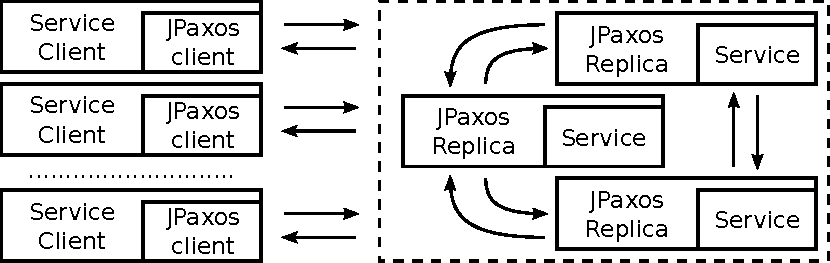
\includegraphics[width=0.44\textwidth]{architecture/userArchitecture1.pdf}
  &
  \hspace{0.02\textwidth}
  &
  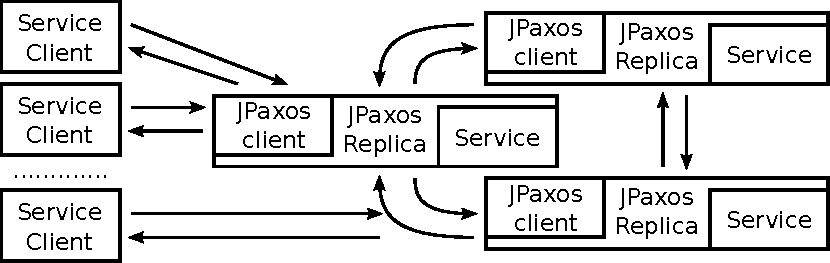
\includegraphics[width=0.44\textwidth]{architecture/userArchitecture2.pdf}
  \\ 
  \scriptsize a) JPaxos client integrated with service client
  & & 
  \scriptsize b) JPaxos client integrated with the replica\\
 \end{tabular}
 \fcmfcaption{Two models of JPaxos}\label{fig:jpaxos_processes}
\end{figure}

The JPaxos \texttt{Client} is responsible for connecting to replicas, providing availability of service as the replica connected with the client crashes, and ensuring that the request will be eventually answered.

Integrating the \texttt{Client} module with the service client provides full transparency of replication for the clients.
The service client contacts with the JPaxos \texttt{Client} module as if it would contact the service, i.e. it executes requests and gets answers for them.

If one chooses the second approach -- i.e. integrating \texttt{Client} in the replica, the transparency is lost, and the programmer must take care for selecting a working replica himself. However, this approach enables using JPaxos in a wider context. For example, one could possibly create a REST web service, and use a usual web client as the service client, while the service itself would be replicated using JPaxos.

The JPaxos Replica module is responsible for global request ordering, passing the requests to the service, answering to the clients and recovering service from crash.

The service itself must be integrated within JPaxos replica. Service gets the requests and returns the response. However, in order to make the resource usage bounded, JPaxos requires additional functionality from the service. This partially breaks transparency -- the service must provide periodically snapshots of it's state, as well as be able to recover it's state from a snapshot, possibly made by other replica.
As we assume that services are deterministic, recovering from snapshot originating from other replica is not a problem. However for some services creating a snapshot may present a challenge.

\subsection{Client and client-replica communication}

The JPaxos client module is a single, light-weight module that performs several tasks:

\begin{tightList}[\setlength{\topsep}{0pt} \setlength{\partopsep}{0pt}]
 \item[\textbullet] Connects to the replicated service
 \item[\textbullet] Reconnects automatically to the replicated service if the connection is lost
 \item[\textbullet] Retrieves (or acknowledges) a client ID for recognising the requests
 \item[\textbullet] Sends the requests
 \item[\textbullet] Waits for answer, retransmitting the request if needed
\end{tightList}

\noindent For the communication with replicas, the client module uses TCP protocol.

\subsection{Service}

% TODO More information about service, service proxy, service interface, service module

The Service module is the core part -- in fact it is the service that uses JPaxos for replication.
In order to integrate a service with the library, it must implement an interface specified in JPaxos. The interface provides required communication between the library and the service.

The interface for interconnecting JPaxos replica and service allows for:
\begin{tightList}
 \item[\textbullet] Executing requests and providing answers for them
 \item[\textbullet] Creating snapshots
 \item[\textbullet] Recovering from snapshots
\end{tightList}

\subsection{Replica}

Replica is the most important part of JPaxos. It consists of numerous modules as depicted in figure \ref{fig:replica_architecture}.

\begin{figure}[h]
 \centering
 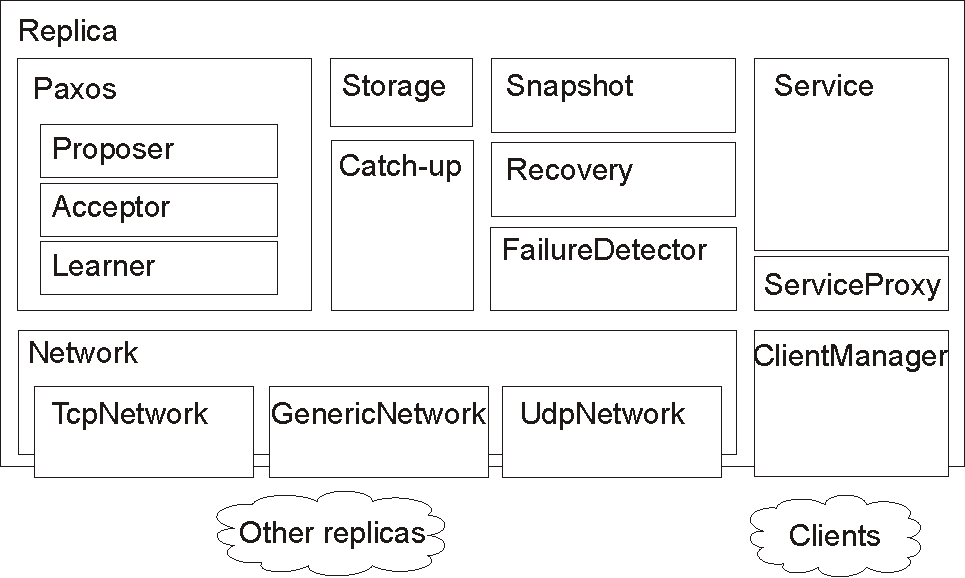
\includegraphics[keepaspectratio, width=0.75\textwidth]{architecture/replica_architecture.pdf}
 \caption{Block diagram of JPaxos modules}
 \label{fig:replica_architecture}
\end{figure}

Short description of the JPaxos modules goes as follows:

\begin{description}
  \item[Replica ] interconnects other modules -- especially the ClientManager, Paxos ans ServiceProxy
  \item[ClientManager ] maintains connection to clients, receives requests from them and forwards the answers
  \item[Paxos ] implements the MultiPaxos consensus algorithm
  \begin{description}
    \item[Proposer ] sends new proposes
    \item[Acceptor ] receives proposes and accepts them
    \item[Learner ] collects accepts and decides
  \end{description}
  \item[CatchUp ] takes care for lost ballots and retrieves the state from others on recovery
  \item[SnapshotMaintainer ] controls the snapshot mechanism
  \item[Recovery ] chooses a proper recovery method and does the actual recovery processes
  \item[Storage ] keeps the state of the Paxos protocol, i.e. view number, log of consensus instances and a snapshot
  \item[Service Proxy ] contacts with the user defined Service, provides as much trans\-pa\-rency as possible for the service
\end{description}

\section{Storage and data structures}
\label{sec:storage_and_data_structures}

Apart of modules and interaction among them it is important to choose proper routines to access data. Both within modules as well as data shared across whole JPaxos.% TODO not English

\subsection{Process descriptor}

Every application has some configurable options that stay unchanged during the run. In JPaxos all these constants are kept in the \texttt{ProcessDescriptor} class.

During the system startup, JPaxos reads a configuration file and initializes ProcessDescriptor with proper values for:
\begin{tightList}[\setlength{\labelwidth}{0em}]
 \item[\textbf{crashModel}] the crash model (see chapter \ref{chapter:recovery})
 \item[\textbf{logPath}] path for the stable storage
 \item[\textbf{localId}] the number of replica % TODO
 \item[\textbf{numReplicas}] count of the replicas % TODO
 \item[\textbf{windowSize}] a preferred window size (see \ref{subsec:concurrent_instances})
 \item[\textbf{batchingLevel}] a maximum size of the batch (see \ref{sec:batching})
 \item[\textbf{maxBatchDelay}] delay for connecting requests for batching in milliseconds
 \item[\textbf{network}] network protocol to be used (TCP or UDP)
 \item[\textbf{maxUdpPacketSize}] a threshold for generic network
\end{tightList}

\subsection{Storage interface}
\label{subsec:storage_interface}

\texttt{Storage} interface is responsible for holding the data for the Paxos protocol.

The data is shared across various modules.
It is very likely that various threads might want to access the \texttt{Storage} simultaneously. In order to prevent concurrency-related errors only one thread, the Dispatcher, may access these data. So if one wants to modify the \texttt{Storage}, a proper \texttt{Runnable} must be passed to the Dispatcher for execution (see subsection \ref{sec:threads}).

\paragraph{\normalfont \ttfamily Storage}
holds the data as follows:
\begin{tightList}[\setlength{\labelwidth}{0em}]
  \item[\textbf{log}] the Paxos Log (see section \ref{subsec:the_paxos_log})
  \item[\textbf{view}] current view
  \item[\textbf{firstUncommitted}] first instance not decided yet instance.
  \item[\textbf{windowSize}] the current size of the window used for multiple instances
  \item[\textbf{acceptors}] a list of processes acting as acceptors
  \item[\textbf{snapshot}] the most recent snapshot
  \item[\textbf{epoch}] the current epoch vector (see section \ref{sec:epoch_ss})
\end{tightList}

\strut

The type of \texttt{Storage} implementation must be chosen according to requirements impose by the model or recovery.
The implementation decides which elements must be kept in the stable storage and which may be placed in volatile memory.

\subsection{The Paxos Log}
\label{subsec:the_paxos_log}
The most important data structure for Paxos, the Log, is part of the \texttt{Storage}.
In our program responsible for that is the \texttt{Log} interface and the \texttt{Con\-sen\-susInstance} class.

\texttt{ConsensusInstance} is a class keeping all data related to a single instance of Paxos: % TODO
\begin{tightList}[\setlength{\itemindent}{0pt}\setlength{\leftmargin}{2\leftmargin}]
  \end{tightList}
  \item[\textbf{view}] a view of the last received message related with this instance,
  \item[\textbf{value}] the value which is held by this instance (i.e. packed requests that are received from clients and executed after deciding), %TODO deciding what
  \item[\textbf{state}] the instance can be in one of three states:
  \begin{tightList}[\setlength{\itemindent}{0pt} \setlength{\labelwidth}{7em}]
    \item[\texttt{\tiny UNKNOWN}] no information about the value of this instance,
    \item[\texttt{\tiny KNOWN}] a view and value are specified and \textbf{can} be changed later,
    \item[\texttt{\tiny DECIDED}] a value is already chosen and \textbf{cannot} be changed.
  \item[\textbf{accepts}] set of known replicas which acceptedthe (view, value) pair.
\end{tightList}

Theoretically \texttt{Log} should contain all instances from the first up to the current one. Of course, the implementation cannot provide this. The log must however contain all instances between the oldest still needed and current one. Only method that guarantees bounding the log (i.e. that count of needed instances will stay finite) is the ability to record a state of the Service periodically -- we call this functionality snapshotting (see \ref{sec:snapshotting}). % TODO rewrite

The \texttt{Log} implementation always keeps all instances with id between \textbf{lowestAvailableId} (inclusive) and \textbf{nextId} (exclusive). Instances below \textbf{lowestAvailableId} have already been truncated and instances above \textbf{nextId} are yet unknown. %TODO define lowestAvailableId

New instances can be appended to the log and after this operation \textbf{nextId} value is increased by 1. \\Log also allows to retrieve instances from it. There are three possible cases when retrieving an instance with a specified id:
\begin{itemize}
  \item (id $<$ lowestAvailableId) -- instance has been truncated and null value is returned,
  \item (lowestAvailableId $\leq$ id $<$ nextId) -- instance is inside log so it is returned,
  \item (nextId $\leq$ id) -- empty instances between nextId and id are created and an empty instance is returned.
\end{itemize}
Old instances can be removed by truncating the log and after that lowestAvailableId is increased. 

Appending, retrieving and truncating instances are three main operations per\-for\-med by log.

\subsection{Significant data structures}
% TODO is the Thesis reader able to understand what are these?
% it it information for the JPaxos "user" or "developer"? Or it's documentation of JPaxos design


Other noteworthy data structures include:
\label{subsubsec:significant_structures}
  \begin{description}
    \item[pendingRequests Map\textless RequestId, ClientId\textgreater] Keeps the requests received from the client for execution that were not yet executed. After execution of request, the reply is sent to client from this structure.
    \item[lastReplies Map\textless ClientId, Reply\textgreater] For each client, keeps the last reply that was sent to it. If client retransmits message which was executed, replica responses immediately.
    \item[decidedWaitingExecution Map\textless Integer, BatchedRequests\textgreater] Paxos might decide in\-stan\-ce $k$ before instance $k-1$, but the replica must execute all requests in order. So it must cache in\-stan\-ce $k$ until all previous instances are decided.
    \item[executedRequests Map\textless ClientId, Reply\textgreater] We have to save IDs of all requests which were executed on state machine to prevent executing the same request twice.
	\item[executedDifference Map\textless Integer, Replies\textgreater] Used to recreate executedRequests stru\-ctu\-re for moment when snapshot was made by state machine.
  \end{description}



\section{Threads}
\label{sec:threads}

A proper design of a multi-threaded application % TODO what application
must contain description of the major threads, their responsibilities and interactions. 

\begin{description}
  \item[Replica] \hfill
    
    Designed as an event loop. The thread % TODO what thread
    waits for new events at certain event queue and reacts on them.

    An event may either be a signal from Paxos about a new decision, or it may concern snapshotting, e.g. a new snapshot was made by service, the catch-up provided a new snapshot or a new snapshot has been requested from the service.

    For most of the time Replica thread waits for requests to be ordered. If they can not be executed yet, it puts them on a list (it uses for that % TODO ??
    the decidedWaitingExecution object).
    
    As for snapshotting -- the thread is a proxy ensuring linearizability in snapshot handling.
    Multiple threads (replica itself, dispatcher and catch-up) may therefore safely execute their snapshot-concerning routines.
    
  \item[Dispatcher] \hfill \nopagebreak
    
    Also designed as an event loop, the dispatcher executes the Paxos consensus algorithm as well as provides secure access to critical data structures -- to the \texttt{Storage} (see subsection \ref{subsec:storage_interface}).
    
    The Dispatcher thread is using a priority queue, so that the events are sorted by their importance -- for example, writes to the storage and the Paxos-related processing events have a higher priority than the Catch-Up tasks.
    
    The dispatcher is responsible for sending, receiving and handling most of protocol messages as well as accessing the \texttt{Storage} and triggering Catch-Up.
    
    Events are placed in the event queue in the following situations:
    

    % TODO methods? that generate these events or what?
    \begin{tabular}{rl}
      Recovery.NetworkListener & \begin{tabular}[t]{l}
                          received a new message \\
                          sent a message
                        \end{tabular} \\
      FailureDetector & \begin{tabular}[t]{l}
                          suspects another process \\
                          leader sends alive messages
                        \end{tabular} \\
      Paxos.NetworkListener & \begin{tabular}[t]{l}
                          received a new message \\
                          sent a message
                        \end{tabular} \\
      Paxos.propose() & \begin{tabular}[t]{l}
                          the application starts a new proposal
                        \end{tabular} \\
      Paxos.startProposal() & \begin{tabular}[t]{l}
                                the application asks the current process \\ \hspace{1em} to become a proposer.
                              \end{tabular} \\
      Proposer &  \begin{tabular}[t]{l}
                    timeout for requests to be batched
                  \end{tabular} \\
      Retransmitter & \begin{tabular}[t]{l}
                        message should be retransmitted
                      \end{tabular} \\
      Catch-Up &  \begin{tabular}[t]{l}
                   gets and merges log fragment \\
                   a message is received \\
                   received a snapshot form other replica \\
                   a periodcal catch-up should occur
                 \end{tabular} \\
      SnapshotMaintainer & \begin{tabular}[t]{l}
                             truncates the log after receiving new snapshot
                           \end{tabular} \\
    \end{tabular}


        % TODO What are these? (we should better describe what we want to present in this section and why)
	\item[NioClientManager] \hfill

		By using java.nio package, we only need one thread \textsc{SelectorThread} to manage all clients connection. Every time a new event occurs (an incoming connection waits for accepting, data received from client, data ready to be sent) an appropriate action is executed. The current implementation allows easy scaling % TODO ??
                to more \textsc{SelectorThread}'s to balance the CPU load if one thread wouldn't cope with a large number of connections.

	\item[UdpNetwork] \hfill

		One thread responsible for listening on DatagramSocket for datagram packages. Every time a new message is received, it is deserialised and all listeners are notified. 

	\item[TcpNetwork] \hfill

		For TCP connection between each two replicas a separate thread for receiving and transmitting is created. Also there is one thread which waits for new incoming connections. Overall we have  $2 \cdot \text{\textit{replica count}} - 1$ % TODO explain this in more detail
                threads handling TCP. Each of them can be in one of three states:
		\begin{itemize}
			\item connected, waiting for new messages,
			\item not connected, trying to establish a new connection,
			\item waiting for a new connection to be established by other replica.
		\end{itemize}
\end{description}
